\xclearpage


%\chapter{\CoP\,-- A Survey of Important Results}
\chapter[COP -- A Survey]{Consecutive-ones Property -- A Survey of
  Important Results} 
\label{ch:copsurvey}

This chapter surveys several results that are significant to this
thesis or to \COP in general. These predominantly pertain to
characterizations of \COP, algorithmic tests to check for \COP (COT),
optimization problems on binary matrices that do not have \COP and
some applications of \COP.

\tnote[dire]{ADD: have a few lines about organization of chapter}


\section{\COP in Graph Theory}

\COP is closely connected to several types of graphs by way of
describing certain combinatorial graph properties. There are also
certain graphs, like convex bipartite graphs, that are defined solely
by one of its associated matrix having \COP.  In this section we will
see the relevance of \cop to graphs.  To see this we introduce certain
binary matrices that are used to define graphs in different
ways. While adjacency matrix is perhaps the most commonly used such
matrix, Definition~\ref{def:graphmatrices} defines this and a few
more.

\begin{definition}
  {\em Matrices that define graphs. \cite[Def.~2.4]{d08phd}.}  
  \label{def:graphmatrices} 
  Let $G$ and $H$ be defined as follows. $G = (V,E_G)$ is a graph with
  vertex set $V = \{v_i \mid i \in [n]\}$ and edge set $E_G \subseteq
  \{(v_i,v_j) \mid i, j \in [n]\}$ such that $|E_G| = m$. $H = (A, B,
  E_H)$ is a bipartite graph with partitions $A = \{a_i \mid i \in
  [n_a]\}$ and $B = \{b_i \mid i \in [n_b]\}$.
  \begin{enumerate}[{\ref{def:graphmatrices}}--i.]
  \item \emph{Adjacency matrix} of $G$ is the symmetric $n \times n$
    binary matrix $M$ with $m_{i,j} = \un$ \iff $(v_i,v_j) \in E_G$
    for all $i,j \in [n]$.
  \item \emph{Augmented adjacency matrix} of $G$ is obtained from its
    adjacency matrix by setting all main diagonal elements to \un, \ie
    $m_{i,i} = \un$ for all $i \in [n]$.
  \item \emph{Maximal clique matrix} or \emph{vertex-clique incidence
      matrix} of $G$ is the $n \times k$ binary matrix $M$ with
    $m_{i,j} = \un$ \iff $v_i \in C_j$ for all $i \in [n], j \in [k]$
    where $\{C_j \mid j \in [k]\}$ is the set of maximal cliques of
    $G$.
    \label{def::maxcliquematrix}
  \item \emph{Half adjacency matrix} of $H$ is the $n_a \times n_b$
    binary matrix $M$ with $m_{i,j} = \un$ \iff $(a_i, b_j) \in E_H$.
  \end{enumerate}
\end{definition}

\figgraphmatrices

Now we will see in Definition~\ref{def:graphwithcop} certain graph
classes that is related to \COP or \CROP.\\

\begin{definition}{\emph{Graphs that relate to
      COP.\cite[Def.~2.5]{d08phd}}} %
  \label{def:graphwithcop} %
  Let $G$ be a graph and $H$ be a bipartite graph.
  \begin{enumerate}[\ref{def:graphwithcop}--i.]
  \item $G$ is \emph{convex-round} if its adjacency matrix has the
    \CROP.
  \item \label{def::concave-round} $G$ is \emph{concave-round} if its
    augmented adjacency matrix has \CROP. \tnote[pressing]{cite BHY00}
  \item $G$ is an \emph{interval graph} if its vertices can be mapped
    to intervals on the real line \stt two vertices are adjacent \iff
    their corresponding intervals overlap \tnote[pressing]{cite Ben59,
      Haj57}.  $G$ is an interval graph \iff its maximal clique matrix
    has COP \cite{fg65}\footnote{This follows \cite{gh64} which states
      that the maximal cliques of interval graph $G$ can be linearly
      ordered \stt for all $v \in V(G)$, cliques containing $v$ are
      consecutive in the ordering \cite[Th. 8.1]{mcg04}.}
    \begin{enumerate}[a.]
    \item $G$ is a \emph{unit interval graph} if it is an interval
      graph \stt all intervals have the same length.\footnotemark[2]
    \item $G$ is a \emph{proper interval graph} if it is an interval
      graph \stt no interval properly contains another.\footnote{The
        set of unit interval graphs and the set of proper interval
        graphs are the same} \tnote[pressing]{cite {rob69,gar07} in
        footnote. pg 33 dom}
    \end{enumerate}
 \item $G$ is a \emph{circular-arc graph} if its vertices can be
    mapped to a set of arcs on a circle \stt two vertices are adjacent
    \iff their corresponding arcs overlap.\tnote[pressing]{how is
      CO/ROP related?}
  \item $H$ is \emph{convex bipartite on columns (rows)} if its half
    adjacency matrix has \COP on rows (columns).%
    \label{def::convexbi}
  \item $H$ is \emph{biconvex bipartite} or \emph{doubly
      convex}\cite{yc95} if its half adjacency matrix has \COP on both
    rows and columns.
  \item $H$ is \emph{circular convex} if its half adjacency matrix has
    \CROP.
  \end{enumerate}
\end{definition}

Interval graphs\footnote{\cite{mcc04} cites that the problem of
  recognizing interval graphs has significance in molecular
  biology. Interestingly, in the late 1950s, before the structure of
  DNA was well-understood, Seymour Benzer was able to show that the
  intersection graph of a large number of fragments of genetic
  material was an interval graph \cite{sb59}. This was regarded as
  compelling evidence that genetic information was somehow arranged
  inside a structure that had a linear topology which we now know to
  be true from the discovery of linear structure of DNA.}and
circular-arc graphs have a long history in research.  The interest
around them is due to their very desirable property that several
problems that are NP-complete on general graphs, like finding a
maximum clique or minimum coloring or independent set, are polynomial
time solvable in these graph classes \cite{clrs01}.  In a similar
fashion, a lot of problems that are hard on general matrices have
efficient solutions on matrices with \COP or \CROP \cite[more
citations pg.\,33]{d08phd}.

Table~\ref{tab:graphmatrices} summarises the way these graphs are
characterized by their matrices having \COP or \CROP.
Our focus in this chapter (and thesis) is mainly \COP and 
having seen how useful \COP is in identifying or characterizing many
types of graphs, we will now see results that study recognition of \COP
in matrices in the following section.

\tabgraphmatrices  

\section{Matrices with COP}
\label{sec:surveycoptest}

The most important questions with respect to a particular 
property desired in a structure/object are perhaps the following.
\begin{itemize}%[]
\singlespacing
\item Does the desired property exist in the given input?
\item If the test is affirmative, what is a certificate of the affirmative?
\item If the test is negative, what are the optimization possibilities
  for the property in the input? In other words, how close to having the
  property can the input be?
\item If the test is negative, what is a certificate of the negative?
\end{itemize}

In this section and the rest of the chapter we see results that shaped the
correponding areas respectively for \cop in binary matrices.

\begin{enumerate}[a.]
\singlespacing
\item \label{q:testcop} Does a given binary matrix have \COP?
\item \label{q:copperm} What is the \COP permutation for the given matrix with \COP?
\item \label{q:copopt} What are the optimizations possible and practically useful on
  the given matrix without \COP?
\item \label{q:nocopcert} If algorithm for (\ref{q:testcop}) returns
  \textbf{false}, can a certificate for this be computed?
\end{enumerate}

Without doubt, besides computing answers to these questions, we are
interested in the efficiency of these computations in terms of
computational complexity theory. Results towards
questions~(\ref{q:testcop}) and (\ref{q:copperm}) are surveyed in this
section. Those for question~(\ref{q:copopt}) are discussed in
Section~\ref{sec:surveycopopt} and question~(\ref{q:nocopcert}) is discussed
in Section~\ref{sec:surveycertalgo}.

It may be noted that one way to design an algorithm to test for \COP
is by deriving one from any interval graph recognition algorithm using
the result \cite{hmpv00} \cite[Th~2.7]{d08phd} which demonstrates how
such a derivation can be done. However, this does not necessarily
yield an efficient algorithm. We will see results that directly solve
the problem on matrices since it is known that
questions~(\ref{q:testcop}) and (\ref{q:copperm}) stated above for
\COP are efficiently solvable.  Table~\ref{tab:cophistory} gives a
snapshot of these results.

\tabcophistory

The first polynomial time algorithm for \COP testing was by
\cite{fg65} which uses overlapping properties of columns with \un
s. Their result has close relations to the characterization of
interval graphs by \cite{gh64}. A graph $G$ is an interval graph \iff
all its maximal cliques can be linearly ordered \stt for any vertex
$v$ in $G$, all the cliques that $v$ is incident on are consecutive in
this order. Clearly, this means that the maximal clique incidence
matrix\footnote{
  Definition~\ref{def:graphmatrices}~\ref{def::maxcliquematrix}} must
have \COP on rows.

A few years later, a deeply significant result based on very different
ideas in understanding \COP came from Tucker which gave a
combinatorial (negative) characterization of matrices with COP
\cite{at72}. This result influenced most of the \COP results that
followed in the literature including linear time
algorithms\tnote[pressing]{linear? did it? which ones?} for \COP
recognition.


\subsection{Tucker's forbidden submatrices for \COP}
\label{sec:tucker}

\cite{at72} discovered certain forbidden structures for convex
bipartite graphs\footnote{The terminology in \cite{at72} differs. It
  uses the term {\em graphs with $V_1$-consecutive arragement} instead
  of {\em convex bipartite graphs}.} and by definition of this graph
class, this translates to a set of forbidden submatrices for matrices
with \cop.  The following are the theorems from \cite{at72} that
acheived this characterization.


Theorem~\ref{th:tuckeratfree} states that convex bipartite graphs
cannot have {\em asteroidal triples}\footnote{If $G = (V,E)$ is a
  graph, a set of three vertices from $V$ form an {\em asteroidal
    triple} if between any two of them there exists a path in $G$ that
  does not contain any vertex from the closed neighborhood of the
  third vertex.} contained in the corresponding vertex
partition\footnote{The partition corresponds to columns (rows) if its
  half adjacency matrix has \COP columns (rows).}.
Theorem~\ref{th:tuckerforbidden} lists the structures in a
bipartite graph that force one of its vertex partitions to have
asteriodal triples -- in other words, it identifies the subgraphs that
prevent the graph from being convex bipartite.


\begin{theoremsansproof}
  [{\cite[Th.~6]{at72}, \cite[Th.~2.3]{d08phd}}]%\\
  A bipartite graph $G = (V_1, V_2, E)$ is convex bipartite on
  columns\footnote{Abridged to match terminology adopted in this
    document. See previous note.} \iff $V_1$ contains no asteroidal
  triple of $G$.
  \label{th:tuckeratfree}
\end{theoremsansproof}

\begin{theoremsansproof}
  [{\cite[Th.~7]{at72}, \cite[Th.~2.4]{d08phd}}]%\\
  In a bipartite graph $G = (V_1, V_2, E)$ the vertex set $V_1$
  contains no asteroidal triple \iff $G$ contains none of the graphs
  $G_{I_k}$, $G_{II_k}$, $G_{III_k}$ (with $k \ge 1$), $G_{IV}$,
  $G_{V}$ as shown in Figure~\ref{fig:forbiddensubgraphs} as subgraphs.
  \label{th:tuckerforbidden}
\end{theoremsansproof}


\figforbiddensubgraphs


Theorem~\ref{th:tuckeratfree} and Theorem~\ref{th:tuckerforbidden}
result in the following Theorem~\ref{th:tuckercop} which characterizes
matrices with \COP.

\begin{theoremsansproof}
  [{\cite[Th.~9]{at72}, \cite[Th.~2.5]{d08phd}}]%\\
  A matrix $M$ has \COP \iff it contains none of the matrices 
$M_{I_k}$, $M_{II_k}$, $M_{III_k}$ (with $k \ge 1$), $M_{IV}$,
  $M_{V}$ as shown in Figure~\ref{fig:forbiddensubmatrices} as submatrices.
  \label{th:tuckercop}
\end{theoremsansproof}

\figforbiddensubmatrices

It can be verified that the matrices in
Figure~\ref{fig:forbiddensubmatrices} are the half adjacency matrices
of the graphs in Figure~\ref{fig:forbiddensubgraphs} respectively
which is not surprising due to
Definition~\ref{def:graphwithcop}~\ref{def::convexbi}.

\subsection{Booth and Lueker's $PQ$-tree -- a linear COT algorithm} %[\PQtree]

Booth and Lueker in their paper \cite{bl76} gave the first linear
algorithm\footnote{Time complexity is $O\left(m+n+f\right)$ where $m
  \times n$ is the order of the input matrix and $f$ is the number of
  $\un$s in it.} for \cop testing while given a linear time interval
graph recognition algorithm by a simplification of \tnote[important]{cite -
  A. Lempel, S. Even and I. Cederbaum, An Algorithm for Planarity
  Testing of Graphs, Theory of Graphs, ed., P. Rosenstiehl, Gordon and
  Breach, New York, (1967), 215-232.  }'s planarity test algorithm.
% Hsu in wlh01 said BL76 gave a planarity test - "the induced PQ-tree
% algorithm can considerably simplify Booth and Lueker’s modification
% of Lempel, Even and Cederbaum’s planarity test. " 
%
% McConnell in hm03 said the first linear algo for interval graph
% recog was by BL76 - "Benzer’s work and other applications of
% interval graphs motivated a search for efficient algorithms for
% recognizing interval graphs, and for constructing a set of intervals
% to represent the graph when it is one [8]. A linear-time algorithm
% was given in 1976 by Booth and Lueker [2]." 
\cite{bl76} introduces a data structure called \PQtree and their \COP
testing algorithm is a constructive one that outputs a \PQtree if the
input has \COP. A \PQtree represents all the \COP orderings of the
matrix it is associated with. \cite{bl76}'s algorithm uses the fact
that if a matrix has \COP, a \PQtree for it can be constructed. It is
interesting to note that aside from interval graph recognition and
\COP testing, \PQtree is also useful in other applications like
finding planar embeddings of planar graphs \cite{lec67,mcc04} and
recognizing \CROP in a matrix.

%\begin{minipage}[h]{5.5in}
\begin{definition}[\PQtree \cite{bl76, mcc04}]
  A \PQtree of matrix $M$ with \COP on columns (rows), is a tree with
  the following properties.
  \begin{enumerate}[i.]
    \singlespacing
  \item Each leaf uniquely represents a row (column) of $M$. The leaf
    order of the tree gives a \COP order for column (row)\footnote{Note
      that \COP order for column requires permutation of rows and vice
      versa.} for $M$.
  \item Every non-leaf node in the tree is labeled $P$ or $Q$.
  \item \label{def::nodep} The children of $P$ nodes are
    unordered. They can be permuted in any fashion to obtain a new
    \COP order for $M$.
  \item \label{def::nodeq} The children of $Q$ nodes are linearly
    ordered. Their order can be reversed to obtain a new \COP
    order for $M$.
  \end{enumerate}
  \label{def:pqtree}
\end{definition}
%\end{minipage}

See Figure~\ref{fig:pqtree} for an example of \PQtree. It may be noted
that there is no way an empty set of \COP orderings can be represented
in this data structure. For this reason, \PQtree is undefined for
matrices that do not have \COP.  Thus effectively, there exists a
bijection between set of matrices with \COP and the set of \PQtrees
(accurately speaking, each matrix with \COP bijectively maps to an
equivalence class of \PQtrees resulting from properties (\ref{def::nodep}) and
(\ref{def::nodeq})).


\figpqtree

The \cite{bl76} algorithm with input $n \times m$ matrix $M$ starts
with a \PQtree for a vacuous $n \times 0$ matrix $M'$ (submatrix
induced by 0 columns). This is known as a {\em universal} \PQtree
which is one with its root as a $P$ node and only leaves as its
children -- each leaf representative of a row of input (by definition
of \COP for columns). This induced submatrix $M'$ vacuously has \COP.
Each column is then added iteratively to $M'$ to check if the new $M'$
has \COP.  By a complicated, but linear, procedure the algorithm does
one of the following actions in each iteration: (a) declare that $M$
has no \COP, or (b) modify the current \PQtree to represent the new
$M'$ (which clearly, must have \COP, since if not, option (a) would
have been executed).


Judging from notes in literature, this algorithm is apparently
notoriously difficult to program. In the procedure to modify the
\PQtree at each iteration, nodes are considered from leaves to
tree. At each node considered, it uses one of nine templates to
determine how the tree must be altered in the vicinity of this
node. Recognition of this template poses a difficult challenge in
terms of implementing it. Each template is actually a representative
of a larger class of similar templates, which must be dealt with
explicitly by a program\cite{mcc04}.


After the invention of \PQtrees, presumably due to the implementation
challenge it posed, there has been several variants of the same in the
literature, like \PCtree \cite{sh99,wlh01,hm03}, generalized \PQtree
\cite{km89,mcc04}, \PQRtree \cite{mm96,mpt98} etc. Most of these are
generalizations of \PQtree\ -- for instance, \PCtree is generalized to
matrices with \CROP, \PQRtree and generalized \PQtree are generalized
to matrices and set systems with or without \COP. \cite{km89} invented
a modified form of \PQtree a simpler incremental update of the tree
only for recognizing interval graphs.  \cite{kr88} constructed
efficient parallel algorithms for manipulating \PQtrees. \temptext{dom
  chapter 2 pg 40 Variations of PQTrees first para - summarize.}

In the next few sections we will see some of these
variations.
%Their algorithm was improved by \cite{tm05}
%\tnote{improved in terms of what?}. 
% describes an improved algorithm to
% build PQR trees.




\subsection{\PQRtree\ --  COP for set systems}
\label{sec:surveycertalgo}

Section~\ref{sec:motive} mentions how a binary matrix naturally maps
to a system of sets.  A set can be constructed for each column of
matrix with its elements being those row indices at which the column
has \un s. Thus the collection of sets corresponding each column of
the matrix forms a set system with universe as the set of all row
indices of the matrix.  This simple construction is formally described
in Definition~\ref{def:matrixsetsystem} along with the idea of \cop
for set systems\footnote{As seen in Section~\ref{sec:courseschedule}}.

\begin{definition}[{\em \Cop for set systems}]%
  \label{def:matrixsetsystem}%
  % [\emph{Set system of a binary matrix}.]
  Let $M$ be a binary matrix of order $n \times m$ and $\{c_i \mid i
  \in [m]\}$ be the columns in $M$.  A set system $\cF_{M} = \{S_i
  \mid S_i \subseteq [n], i \in [m]\}$ is defined such that for every
  column $c_i$ of $M$, set $S_i = \{j \mid m_{ji} = \un \}$. The
  collection $\cF_M$ is the {\em set system of binary matrix} $M$. The
  {\em binary matrix for set system} $\cF$ is conversely constructed
  and denoted by $M^\cF$. Thus, $M^{\cF_M} = M$.%
  \par\noindent%
  A set system $\cF$ from universe $U$, $|U| = n$ has the {\em \cop}
  if there exists a linear order or permutation $\sigma = w_1w_2\ldots
  w_n$ that can be applied to $U$ \stt each set $S \in \cF$ becomes a
  consecutive subsequence\footnote{Also termed an {\em interval}}
  $w_{i}w_{i+1}\ldots w_{i+k-1}$ on $\sigma$ for some positive integer
  $i \le n+1-k$ where $k = |S|$.
  \par\noindent%
  The set $\valid{U,\cF}$ respresents all \COP orders of $\cF$ in $U$.
  \dstop
\end{definition}

It is easy to see the equivalence of this definition to \COP for
matrices in Definition~\ref{def:copmatrix}.

Before proceeding to describe \PQRtree per se, we will see a few more
terminologies that will make the subsequent discussion in this section
simpler.

\begin{definition}[\em Orthogonal sets \cite{n89, mm96,
    mcc04}\footnote{\cite{mcc04} does not use the term ``mutually
    orthogonal'' but refers to the same idea as ``sets that do not
    overlap''. This terminology is also used in other literature like
    \cite{nsnrs09,wlh02}.} etc.]
  \label{def:orthosets}%
  Let $\cF$ be a set system with universe $U$ and sets $A, B \in \cF$.
  \begin{enumerate}
  \item $A$ and $B$ are said to have a {\em trivial intersection} if
    $A \cap B$ is one of the following.
    \begin{enumerate}[i.]
    \singlespacing
    \item $\emptyset$
    \item $A$
    \item $B$\footnote{In other words, $A$ and $B$ are either disjoint
        or one is the subset of the other.}
    \end{enumerate}
    % \vspace{-5mm}%

  \item $A$ and $B$ are called {\em mutually orthogonal} or $A$ is {\em
      orthogonal to} $B$ and vice versa, if they have a trivial
    intersection.

  \item {\em Trivial subsets} of a universe $U$, denoted by $\cT(U)$,
    are sets that have trivial intersections with any set in
    $\power{U}$. These sets are $U$, singleton sets in
    $\power{U}$ and $\emptyset$ \cite{n89, mm96}.
    Thus, $\cT(U) = \{U\} \  \bigcup \  \{ \{v\} \mid v \in U \} \  \bigcup \
    \{\emptyset\}$.

  \item {\em Orthogonal sets of a set system} $\cF$ with universe $U$
    are subsets of $U$ that are orthogonal to all sets in $\cF$. The
    set of all orthogonal sets to $\cF$ is denoted by
    $\cF^{\bot}$\footnote{\cite[Def.~3.1]{mcc04} uses the term {\em non-overlapping
    family} of $\cF$ and denotes it by $\cN(\cF)$. \label{mcc1}}.

  \item $\cF$ is called {\em complete}\footnote{\cite{mcc04} calls
      this a {\em weakly partative family}. \label{mcc2}} if the following hold
    true for every pair of non-orthogonal\footnote{Or overlapping.} sets
    $A, B$ in $\cF$.
    \begin{enumerate}[i.]
    \item $\cT(U) \subset \cF$
    \item $A \cup B \in \cF$
    \item $A \cap B \in \cF$
    \item $A \setminus B \in \cF$
    \item $B \setminus A \in \cF$
    \end{enumerate}
    In other words, $\cF$ contains all the trivial
    subsets of $U$, $A \cup B$ and the partitions of $A \cup B$
    defined by intersection and set difference.

  \item $\overline{\cF}$ represents the smallest super set system of
    $\cF$ that is complete\footnote{\cite[Def.~3.2]{mcc04} calls
      this the {\em weak closure} of $\cF$ denoted by
      $\cW(\cF)$. \label{mcc3}}

  \item \label{def::slashop} The binary operator $/$ is defined as
    follows. Let $A, B$ be two sets from set sysetm $\cF$.
    \begin{align*}
      A/B &= A \setminus B \cup \{b\}\\
      \cF/B &= \{ S/B \mid S \in \cF, S \nsubseteq B \}
    \end{align*}
    $b$ is a new element added as a representative for $B$.
 \end{enumerate}
  \dstop
\end{definition}

Generalized \PQtree or \gPQtree is a data structure defined in
\cite{n89} to represent all orthogonal sets of a set system $\cF$. A
data structure with the same name was later defined in \cite{mcc04} as
part of a {\em substitution decomposition} for a set system $\cF$
\tnote[pressing]{define substitutio decomp.} and subsequently \cite{mcc04} gives
a new characterization of $\cF$ using a so-called incompatibility
graph. \PQRtree is defined in \cite{mm96} as a data
structure to represent any set system $\cF$ with additional
information in their $R$-nodes if $\cF$ has no \COP.  All three of
these data structures are proposed as generalizations of \cite{bl76}'s
\PQtree and hence produce the \PQtree if $\cF$ has \COP. As a whole,
all these three data strutures are largely identical with their
differences being notional.  In this section, we will discuss the
basic theory that they all hold. We will predominantly use the
terminology from \cite{mm96} and refer to the data structure as
\PQRtree.

An important observation made by \cite{mm96} is presented now along
with a few theorems that help in decomposing the \COP problem on $\cF$
into subproblems.

\begin{observation}[{\cite[Sec.~3]{mm96}}]
  If $\cF$ is a set system with \COP then, after applying the \COP
  order, not only must every set in $\cF$ be consecutive but the
  following sets must also be consecutive for any $A, B \in \cF$.
\begin{enumerate}
  \item The intersection $A \cap B$ 
  \item The union $A \cup B$ if $A \cap B \ne \emptyset$
  \item The relative complements $A \setminus B$ and $B \setminus A$
    if $B \nsubseteq A$ and $A \nsubseteq B$ respectively.
  \item Also note that trivially, sets in $\cT(U)$ are consecutive in
    any permutation of $U$\footnote{$\emptyset$ is considered
      consecutive by convention.}.
\end{enumerate}
\end{observation}

\temptext{narrative is abrupt from here. add some explanation for the
  theorem and proposition below?}

\begin{theoremsansproof}[{\cite[Th.~3,6]{mm96}}]
  \label{th:validcop}
  For any set system $\cF$ we have the following. \par
  \centering
    $\valid{\cF} = \valid{\overline{\cF}}$ \\
    $\cF^{\bot} = \overline{\cF^{\bot}} = (\overline{\cF})^{\bot}$
\end{theoremsansproof}

\begin{proposition}
  \label{pr:validcop}
  Any set that is consecutive on all the \COP permutations of $\cF$ is
  present in $\overline{\cF}$.
\end{proposition}

Proposition~\ref{pr:validcop} is owing to the following theorem by
which \cite{mm96} describes a way to decompose the problem of finding
all \COP orders of $\cF$ into two subproblems using sets in
$\overline{\cF} \cap \cF^{\bot}$. The operator $/$ used is defined in
Definition~\ref{def:orthosets}~(\ref{def::slashop}).

\begin{theoremsansproof}[{\cite[Th.~7]{mm96}}]
  \label{th:mmdecomp}
  For any set system $\cF$, and $\emptyset \ne H \in \overline{\cF}
  \cap \cF^{\bot}$ we have the following.\par
  \centering
  $\valid{U,\cF} = \valid{U/H,\cF/H} * \valid{H,\cF \cap 2^H}$
\end{theoremsansproof}


\def \ff {\overline{\cF} \cap \cF^{\bot}}
The idea behind Theorem~\ref{th:mmdecomp} is as follows. A permutation $\alpha$
of $U$ is a composition of two permutations with respect to $H$ - (i) a
permutation $\gamma$ of $H$ and (ii) a permutation $\beta$ of $U
\setminus H$.

For two mutually orthogonal sets $A, B$ such that $A \nsubseteq B$,
$A/B$ is defined as the set obtained by removing all elements of $B$
from $A$ and adding a representative element for $B$ in $A$. Being orthogonal,
$A/B$ results in only the following three possibilities.
\begin{enumerate}[i. ]
\item $A$ and $ B$ are disjoint: $A/B  = A$
\item $A$ is a subset of $B$: $A/B$ is not defined
\item $B$ is a subset of $A$: $A/B = A \setminus B \cup \{b\}$, where $b$
is a new element not in $U$ added to represent $B$.
\end{enumerate}

We observe that this idea of decomposing the \COP problem into two
subproblems in \cite{mm96} is very similar to the substitution
decomposition of a set system given in \cite[Sec.~4]{mcc04}.\footnote{Using
  the theory cited in footnotes~\ref{mcc1},\ref{mcc2},\ref{mcc3}.}

The following corollary, Corollary~\ref{cor:pqrrecursive} states how
\PQRtree elegantly fits into this whole theory and help in computing
all \COP orders of $\cF$.

\begin{corollary}[{\cite[Cor.~8]{mm96}}]
  \label{cor:pqrrecursive}
  Let $\cF$ be a set system with universe $U$ and $H$ is a non-empty
  orthogonal set $H \in \ff$. If there is a \PQRtree $T_1$ that
  encodes all permutations in $\valid{U/H, \cF/H}$ and also a \PQRtree
  $T_2$ that encodes all permutations $\valid{H,\cF \cap \power{H}}$,
  then a \PQRtree $T$ for $\cF$ can be obtained by replacing the leaf
  $h$ in $T_1$ by $T_2$, where $h$ is the representative element for $H$.
\end{corollary}

%Finding elements in $\ff$ is done using \PQRtree.

Thus we have a recursive algorithm that can compute the \PQRtree for
$\cF$ provided we find an element from $\ff$ in each iteration. The
non-empty sets in $\ff$ are called {\em node sets} since they form the
nodes in the \PQRtree, as alluded to by
Corollary~\ref{cor:pqrrecursive}. They are calculated as follows.
First method is by computing the overlap components of $\cF$. The
overlap components is the partition that results from the {\em
  overlap} equivalence relation which is nothing but {\em
  non-orthogonal} equivalence relation\footnote{It is easy to verify
  that this relation is indeed an equivalence relation.}. Overlap
components are linearly computable\cite{mm95,wlh92}. Once these
elements are factored out, the rest of the node sets are obtained by
the second method which is identifying {\em twin}
elements\footnote{\cite[Sec.~3]{kklv10} calls this {indistinguishable}
  elements. The equivalence class is called a {\em slot}.}. Two
elements $a, b \in U$ are twins if their membership in every set of
$\cF$ is in tandem with each other, \ie $\{a,b\} \bot \cF$. This is
clearly an equivalence relation and their equivalence classes is known
to be computable in linear time\cite{wlh01,mm96-ref11} and even in
logspace\cite{kklv10}.

The recursion end condition is when one cannot find any more sets from
$\ff$ that are non-trivial. This is when $\ff = \cT(U)$. This is the
point where the parents of the leaves of the final \PQRtree are created. The
following theorem helps the algorithm decide whether a $P$, $Q$ or
$R$ node must be created.

\begin{theoremsansproof}[{\cite[Th.~9]{mm96}}] %,\cite[Th.~2.1]{mcc04}
\label{th:pqrfinalmm}
If $\cF$ is a set system with universe $U$ and $|U| \ge 3$ then one of
the following statements hold.
\begin{enumerate}
\item \label{th::it1} $\overline{\cF} = \cT(U)$ 
\item \label{th::it2}$\overline{\cF} = consec(\alpha)$\tnote[pressing]{what is consec?} for
  some permutation $\alpha$ on $U$ 
\item \label{th::it3}$\overline{\cF} = \power{U}$ 
\end{enumerate}
\end{theoremsansproof}

In case (\ref{th::it1}) of Theorem~\ref{th:pqrfinalmm} all elements in
$U$ are made children of a $P$ node. In case (\ref{th::it2}) all
elements in $U$ are made children of a $Q$ node in the order given by
$\alpha$. Finally, case (\ref{th::it3}) is the situation where no permutation
of $U$ gives \COP. All elements of $U$ are in this case made children
in an $R$ node.

Theorem~\ref{th:pqrfinalmm} and the theory leading to it is very
similar to \cite[esp. Th.~2.1, 3.5. also Th.~3.2, 3.3, 3.4]{mcc04}
which categorizes the nodes in the above the three cases as {\em
  prime}, {\em linear} and {\em degenerate}
respectively. \cite{mcc04}'s generalized \PQtree is created in similar
ways as \PQRtree above. This tree is, in essence, the Hasse diagram of
what they call {\em strong elements} of weak closure,
$\cW(\cF)$\footnote{\ie $\overline{\cF}$}. Strong elements of a set
family are elements that do not overlap with any other elements in the
family, \ie it is orthogonal to all other sets\cite[Def.~3.3]{mcc04}.

\begin{theoremsansproof}[{\cite{mm96}, \cite[Th.~3.6]{mcc04}}]
The set system $\cF$ has \COP \iff its \PQRtree has no $R$ nodes.  
\end{theoremsansproof}

Thus \PQRtree gives a data structure that encodes possible linear
orderings of a set that demonstrates the \COP property in it or
narrows it down to parts of the universe in $R$ nodes that prevent the
set system from having \COP.

As mentioned before, we observe the three data strutures of \PQRtree,
\gPQtree and generalized \PQtree to be equivalent. The terminologies
of the theory of all these data structures is summarised in
Table~\ref{tab:pqrcomparison}.

We will now see, in brief, one more generalization of \PQtree before
seeing another approaches to solving \COP testing called ICPIA which
is a set theoretic characterization of \COP.

\begin{table}[t]
  \def\colwidth{4cm}
  \centering
  \fontencoding{OT1}\fontfamily{cmss}\selectfont%
  \footnotesize%
  \setlength\extrarowheight{0.1in}
  
  \begin{tabular}{l >{\columncolor{\tblhcolor}}l l}
    
    \rowcolor[gray]{0.8} %                 Header row colored
    \normalsize \gPQtree \cite{n89} & 
    \normalsize \PQRtree \cite{mm96} & 
    \normalsize generalized \PQtree \cite{mcc04}
    \\
    
    Trivial intersections &
    Trivial sets $\cT(U)$ & 
    \\\hline
    
    Trivially intersecting sets &
    Mutually orthogonal sets, $A \bot B$ &
    Non-overlapping sets
    \\\hline
    
      &
    Complete collection &
    Weakly partative family
    \\\hline
    
    &
    $\overline{\cF}$&
    Weak closure, $\cW(\cF)$
    \\\hline

    &
    $\cF^{\bot}$&
    Non-overlapping family, $\cN(\cF)$
    \\\hline
    
    &
    \parbox[t]{\colwidth}
    { 
      Sets in $\cF$ orthogonal to all other sets in $\cF$ 
    }&
    Strong elements
    \\\hline

    &
%     \parbox[t]{\colwidth}
%       {}
    \temptext{PQR tree def. }
    &
    \parbox[t]{\colwidth}
    {
      Decomposition tree of $\cW(\cF)$, $T(\cW(\cF))$
      \temptext{PQR tree def. }
    }
    \\\hline

    &
    Node sets, $(\cF \cap \cF^\bot) \setminus \{\emptyset\}$
    \\\hline

    &
    \parbox[t]{\colwidth}
    {
      $P$-node $\Leftrightarrow \cF = \cT(\cF)$\\
      $Q$-node $\Leftrightarrow \cF = consec(\alpha)$\\
      $R$-node $\Leftrightarrow \cF = \power{U}$\\
    }&
    \temptext{give def of P Q R nodes}
    \\\lasthline

  \end{tabular}
  \caption[\figtabsize Comparison of theory of \PQRtree, \gPQtree, generalized
  \PQtree]{\figtabsize Comparison of theory of \cite{mm96} \PQRtree, \cite{n89} \gPQtree,
    \cite{mcc04} generalized \PQtree}
  \label{tab:pqrcomparison}
\end{table}

    
\subsection{\PCtree -- a generalization of \PQtree}

\PCtree is another generalization of \PQtree. It is a data structure that is
analogous to \PQtree but for matrices with \crop. \PCtree was
introduced by \cite{sh99} for the purpose of planarity testing where
this data structure represents partial embeddings of planar
graphs. % noted from wlh01 abstract.
In \cite{wlh01}, Hsu reintroduces \PCtree as a generalization of
\PQtree and shows how it simplifies \cite{bl76}'s planarity test by
making the \PQtree construction much less complicated. Later
\cite{hm03}, discovers that \PCtree is a representation of all \crop
orders of a matrix when it is unrooted. \PCtree presented in
\cite{wlh01} is rooted; however the construction of \PCtree is the
same in both results. The property of being unrooted is necessary in
order to use \PCtree as a data structure for encoding circular
ordering. Definition~\ref{def:pctree} defines \PCtree.

\begin{definition}[\PCtree \cite{wlh01,d08phd}]
  \label{def:pctree}
   A \PCtree of matrix $M$ with
  \CROP on columns (rows), is a tree with the following properties.
  \begin{enumerate}[i.]
    \singlespacing
  \item Is unrooted -- thus it has (a) no parent child relationship
    between nodes (b) there is no left to right (or vice versa)
    ordering.
  \item Each leaf uniquely represents a row (column) of $M$. The leaf
    order of the tree gives a \CROP order for column (row) for
    $M$. Moreover, any sequence obtained by considering the leaves in
    clockwise or counter-clockwise order describes a \CROP order for
    $M$.
  \item Every non-leaf node in the tree is labeled $P$ or $C$.
  \item The neighbors of $P$ nodes can be permuted in any fashion to
    obtain a new \CROP order for $M$.
  \item \label{def::pcmirror} The tree can be changed by applying the following
    ``mirroring'' operation to obtain a new \CROP order for $M$. Root
    the \PCtree at a neighbor of a $C$-node, $v$ and mirror the
    subtree whose root is $v$ and finally unrooting the
    tree. Mirroring a subtree is done by putting the children of every
    node of the subtree in reverse order.
  \end{enumerate}
\end{definition}

\begin{figure}[htbp]
  \centering
  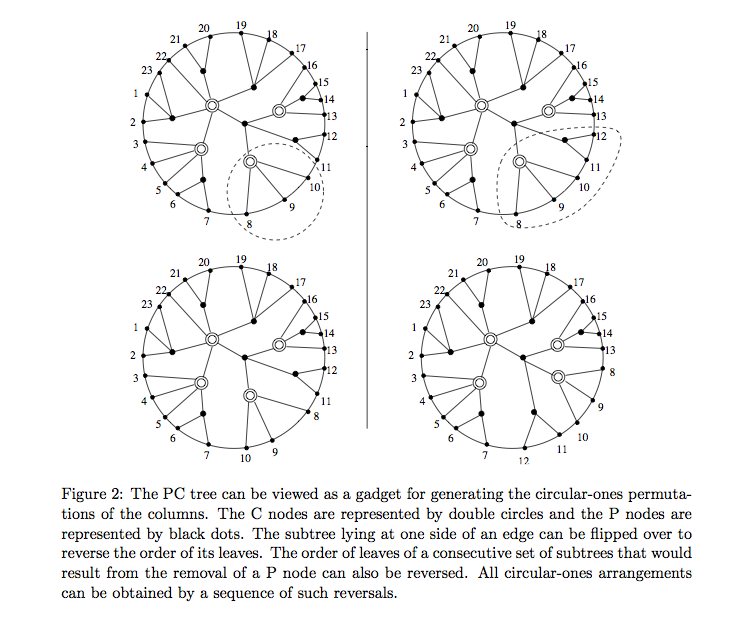
\includegraphics[scale=0.4]{../img/pctree_hm03.png}

  \centering
  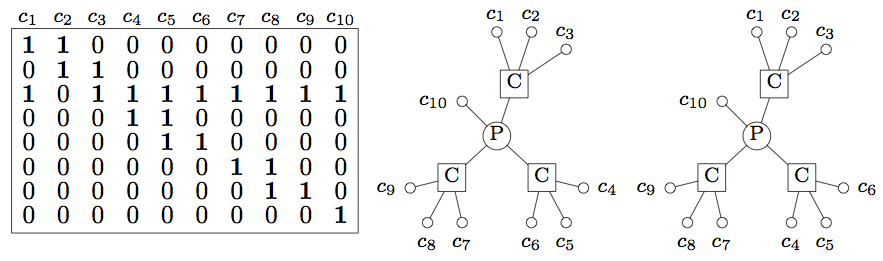
\includegraphics[scale=0.4]{../img/pctree_dom.png}
  \caption{\figtabsize \PCtree \temptext{ PLACEHOLDER 
IMGS \cite{hm03, d08phd}}}
  \label{fig:pctree}
\end{figure}

As a data structure when \PCtree is compared with \PQtree, the
differences are, (i) it is unrooted, (ii) it represents all \CROP order of a
matrix (iii) it has $C$ nodes instead of $Q$ nodes which can be
``mirrored'' (operation defined in Definition~\ref{def:pctree}~\ref{def::pcmirror}).
The algorithms of construction of \PQtree in \cite{bl76} and that of
\PCtree in \cite{wlh01, hm03} starkly differ since the latter is a
much simplified procedure.



% WLH01 abstract:
% [..] The original implementation of the PQ-tree algorithms by Booth and
% Lueker using nine templates in each bottom-up iteration is rather
% complicated. Also the complexity analysis is rather intricate. We give
% a very simple linear time PC-tree algorithm with the following
% advantages: (1) it does not use any template; (2) at each iteration,
% it does all necessary tree-modification operations in one batch and
% does not involve the node-by-node bottom-up matching; (3) it can be
% used naturally to test the circular ones property in matrices; (4) the
% induced PQ-tree algorithm can considerably simplify Booth and Lueker’s
% modification of Lempel, Even and Cederbaum’s planarity test.

% \tnote[FYI]{ The results in cite~{bl76} on COT are based on the
%    result that interval graphs are AT-free chordal graphs cite~{lb62}?
%  No they don't seem related. this is the stupid bl lb confusion.}%



\subsection{ICPIA - a set cardinality based \COP test}
\label{sec:icpiasurvey}
\temptext{narrative is abrupt}

\cite{nsnrs09} describes a characterization of consecutive-ones
property solely based on the cardinality properties of the sets in the
set system and does not use any variants of \PQtrees. 

\begin{definition}[Intersection Cardinality Preserving Interval
  Assignment (ICPIA)]
  \label{def:icpia}
  Let $\cF = \{A_i \mid A_i \subseteq U, i \in [m]\}$ be a set system
  from universe $U$ and the set of ordered pairs $\Pi = \{(A_i, B_i)
  \mid B_i  \text{ is an interval from } [n], i \in [m]\}$ be an {\em interval
    assignment} of $\cF$, then $\Pi$ is called an {\em ICPIA} if it has
  the following properties.
  \begin{enumerate}[i.]
  \item $|A_i| = |B_i|$ for all $i \in [m]$
  \item $|A_i \cap A_j| = |B_i \cap B_j|$ for all $i, j \in [m]$
  \end{enumerate}
\end{definition}

\begin{theoremsansproof}[{\cite[Th.~1]{nsnrs09}}]
  \label{th:icpia1}
  If an interval assignment $\Pi$ is feasible, then it is an ICPIA.
\end{theoremsansproof}

The necessity condition of Theorem~\ref{th:icpia1} is fairly
obvious. It turns out that it is sufficient too.  This is demostrated
by two algorithms which work as follows. The first one iterates over
the assignment $\Pi$ %set system $\cF$
and changes it in each iteration till the altered
assignment %set system
has no more overlapping intervals\footnote{Intervals are the second
  element in each ordered pair of $\Pi$. Def.~\ref{def:icpia}} %sets
\cite[Alg.~1]{nsnrs09}. This is acheived by replacing two overlapping
assignment pairs $(A_i, B_i)$ and $(A_j, B_j)$ with the partitions of
$(A_i \cup A_j,B_i \cup B_j)$ induced by their overlaps -- $(A_i
\setminus A_j, B_i \setminus B_j)$, $(A_i \cap A_j, B_i \cap B_j)$ and
$(A_j \setminus A_i, B_j \setminus B_i)$.

To see it in terms of the theory explained in
Section~\ref{sec:surveycertalgo}, this results in the weak closure of
$\cF$. Let $\cF$, $\cI$ be the set system and interval
system\footnote{A set system where all the sets are intervals.},
respectively, involved in the assignment $\Pi$ and $\cF'$, $\cI'$ be
the same for the output of the algorithm $\Pi'$.  It can be observed
that $\cF' \cup \cF$ is $\overline{\cF}$ or the weak closure of
$\cF$. The analog is true for $\cI \cup \cI'$.  Moreover, this output
$\cF'$, $\cI'$ contains the strong elements of $\overline{\cF}$,
$\overline{\cI}$ respectively. It turns out that $\cI'$ is also an
interval system and that $\Pi'$ is an ICPIA \cite[Lem.~2]{nsnrs09}.

The next algorithm \cite[Alg.~2]{nsnrs09} further refines $\Pi'$ to
$\Pi''$ which represents the family of permutations that yield the
\COP orders represented by $\Pi$ of $\cF$. The subset relation Hasse
diagram of $I'$ is created with each node representing the
corresponding assignment pair of the interval from $\Pi'$. Since all intervals in
$\Pi'$ are non-overlapping, this is a tree. Notice that this means any
two intervals are now either disjoint or one is contained in the
other. Hence this tree is called a {\em containment tree}.  The
algorithm traverses this tree in post order fashion where the post
order function is to replace an assignment pair $(X,Y)$  in $\Pi'$ by their child
assignment pairs in the containment tree, say $(X_1, Y_1),(X_2, Y_2)
\ldots (X_k,Y_k)$. The result $\Pi''$ gives the
\COP order for $\Pi$. These two algorithms prove that ICPIA is a
sufficient condition for the feasibility of the interval assignment.

\begin{theoremsansproof}[{\cite[Th.~2]{nsnrs09}}]
  \label{th:icpia2}
  Let  $\cF = \{A_i \mid A_i \subseteq U, i \in [m]\}$ be a set system
  from universe $U$, $|U| = n$
  and $\Pi = \{(A_i,B_i) \mid B_i \text{ is an interval from } [n], i
  \in [m]\}$ be an ICPIA. Then there exists a permutation $\sigma: [n]
  \rightarrow [n]$ \stt $\sigma(A_i) = B_i$.
\end{theoremsansproof}

What we saw so far in this section is checking for the feasibility of
a given interval assignment. ICPIA can also be used to find an
interval assignment when only the set system $\cF$ is given. Part of
the approach is similar to the overlap component idea in \cite{fg65,
  wlh02}. Once the overlap components are factored out, they can be
independently assigned a subinterval to which the sets in the
component need to be mapped. This is simple because the overlap
components are disjoint from each other. Now the subproblem is finding
\COP order for each overlap component. In each component, the set
whose overlaps with the rest of the sets in that component forms
a single inclusion chain\footnote{A set of sets form a {\em single
  inclusion chain} when the Hasse diagram of their subset relation
forms a single chain. In this particular reference, the set of sets is
the set of overlaps.} is chosen first and assigned the
leftmost\footnote{By convention. Rightmost can also be chosen
  analogously to get a different \COP order.} interval. The next
candidate set is chosen from this set's overlapping sets. The interval
assigned is calculated by simple intersection cardinality
means\footnote{Assume that the next set overlaps on one of the
  ``ends'' of the current set and calculate the interval by shifting
  left or right of the current interval and adjusting its size to
  match the next set's cardinality.}. Once the next set is assigned an
interval, the current assigned sets are all checked for ICPIA. This is
a backtracking algorithm -- if at any point ICPIA fails, another
overlapping set is chosen. If all overlapping set attempts fail ICPIA,
a different ``first set'' is chosen. This is a remarkably simple
algorithm due to its obvious simplicity in implementation.

\subsection{Other \COP testing algorithms}
There are more \COP test algorithms in the literature. We make a
mention of one of them here.  A simple linear time algorithm was
presented by \cite{hmpv00}. They use something called {\em Lex-BFS
  ordering} of the vertices of a graph to decide in linear time
whether the graph is an interval graph. They also show how any
interval graph recognition algorithm can be used to recognize matrices
with \COP. This is shown in Theorem~\ref{th:intgraphcop}.

\begin{theoremsansproof}[{\cite[Th.~2]{hmpv00}}]
  \label{th:intgraphcop}
  For a binary matrix $M$ the following statements are equivalent.
  \begin{enumerate}
  \item The row adjacency graph $G_r(M)$ is an interval graph and $M$
    is its maximal clique matrix.
  \item The columns of $M$ are maximal and $M$ has the \COP for rows.
  \end{enumerate}
\end{theoremsansproof}

\temptext{ abrupt: Add a section closing para. does this method (above)
  lead to efficient algo? }

\section{Optimization problems in COP}
\label{sec:surveycopopt}

\COP is a very beneficial property since it simplifies the structure
of the input\footnote{Binary matrix or set system.} leading to
efficient algorithms to otherwise hard problems.  While
Section~\ref{sec:surveycoptest} discusses matrices with \COP and how
to compute \COP orders, this section describes the problems that are
of interest when a matrix does not have this property.  The central
questions in this area are (i) how close is the matrix to having \COP,
mainly in terms of Tucker's forbidden submatrices, and (ii) how
optimally can one alter the matrix to attain \COP.  With regard to the
latter question, recent literature indicate that there has been a lot
of interest in matrix modification problems to make a matrix have \COP
\cite{hg02, tz07}. However, to tackle this problem it is more than
insightful to solve question (i).

To study the smallest hamming distance \temptext{(?)} between the
input matrix and one with \COP, identifying the Tucker's forbidden
substructures\footnote{See Section~\ref{sec:tucker} for detailed
  discussion on Tucker's forbidden substructures for matrices with
  \COP.} is of prime importance. 

\subsection{Finding forbidden submatrices}
It is known from Theorem~\ref{th:tuckercop}
that when a matrix does not have \COP, it must have one of Tucker's
forbidden submatrices. However, none of the \COP test algorithms discussed in
Section~\ref{sec:surveycoptest} outputs the forbidden submatrix when
the test is negative. This certainly gives a hint to how hard it is to find
these substructures in the input. \temptext{Fill neg results on
  finding forbidden submartrices -- boo75, some highlighted stuff from v85}

In this section we will describe \cite{d08phd}'s approximation
algorithm for finding forbidden submatrix. We will use $\Tuckerset$ to
refer to the set of Tucker's forbidden submatrices shown in
Figure~\ref{fig:forbiddensubmatrices}.


A corollary to one of Tucker's theorems presented in
Theorem~\ref{th:tuckeratfree} is given in
Corollary~\ref{cor:tuckertheorem}. This is central to \cite{d08phd}'s
algorithm.

\begin{corollary}[{\cite[Cor.~3.1]{d08phd}}]
  \label{cor:tuckertheorem}
  A matrix $M$ has \COP \iff its representing bipartite graph
  $G_M$\footnote{Graph whose half adjacency matrix
    (Def.~\ref{def:xxxx}) is $M$.} does not contain an asteroidal
  triple whose three vertices correspond to columns of M.
\end{corollary}




\temptext{
\cite[Ch.~3]{d08phd} describes two main algorithms - one is an
approximation algorithm and the other one is an exact algorithm. 


\begin{theoremsansproof}[{\cite[Th.~3.1]{d08phd}}] 
\label{th:forbiddenalg}
Let $M$ be a $(*,\Delta)$-matrix of size $m
\times n$. A forbidden submatrix from $\Tuckerset$ in $M$ that has a minimum
number of rows can be found in $O(\Delta^3m^2n\dot(m+n^2))$
time. Within the same time, one can also find a forbidden submatrix
from $\Tuckerset$ in $M$ that has a minimum number of columns, a minimum number
of rows and columns, or a minimum number of entries.
  
\end{theoremsansproof}

}


\subsection{Incompatibility graph - a certificate for no \COP}

When a \COP test algorithm reports negative, it is hard to verify
this. While \cite{at72} gives forbidden substructures for \COP, there
are no efficient algorithms to find these strutures in a matrix. In
fact, \cite{v82} shows that even finding a forbidden submatrix with at
least $k$ rows in an input matrix is NP-complete. This was proven by
polynomially reducing the longest path problem for graphs to this
problem.

\cite{mcc04} describes another characterization for matrices without
\COP which is efficiently computable. This is done by way of an {\em
  incompatibility graph} of a set system\footnote{Since \COP in
  matrices and set systems are equivalent problems as seen in
  Section~\ref{sec:surveycertalgo} we will use the term set system
  in this section, in line with \cite{mcc04}'s convention.}. The construction of this graph is based on the following
observation. 

\begin{observation} 
  Consider elements $a, b, c \in U$ and a set system $\cF$ with
  universe $U$. If there is at least one set $S \in \cF$ \stt $a, c
  \in S$ but $b \notin S$, then it is impossible to have a \COP order
  that will place $b$ in between $a$ and $c$. \tnote[important]{also cite the
    inbetweenness problem}
\end{observation}

For the sake of argument, suppose there exists such a \COP
order. Clearly, it will not succeed in mapping $S$ to an interval
since $b \notin S$ which is a contradiction to the assumption that
this is a \COP order.  The ordered pair $(x,y)$ denotes that in the
\COP order $y$ comes after $x$. Based on above observations, this
means $(a,b)$ and $(b,c)$ are not compatible in any \COP order. So are
$(c,b)$ and $(b,a)$.  Thus a binary relation {\em is incompatible
  with} on $U \times U \setminus \{(a,a) \mid a \in U\}$ can be
defined based on the membership of elements of $U$ in the sets in
$\cF$.  \cite{mcc04} creates an incompatiblity graph with vertices
denoting ordered pairs and edges denoting the incompatibility
relation.

\begin{definition}[{\em Incompatibility graph \cite[Def.~6.1]{mcc04}}]
  Let $\cF$ be a set system with universe $U$. Let $A_{\cF} = \{(a,b)
  \mid a, b \in U, a \ne b\}$. The {\em incompatibility graph}
  $G_I^\cF$ of $\cF$ is an undirected graph defined as follows.
%  \singlespacing
  \begin{enumerate}
  \item   The vertex set of $G_I^\cF$ is $ A_{\cF}$
  \item  The edge set of $G_I^\cF$ are pairs of the following forms
    \begin{itemize}
    \item $\{(a,b),(b,a)\}$ for all $a, b \in U$
    \item $\{(a,b),(b,c)\}$ if there exists $S \in \cF$ \stt $a, c
      \in S$ and $b \notin S$, for all $a, b, c \in U$
    \end{itemize}
  \end{enumerate}
  \dstop
\end{definition}

Thus an edge between two vertices $(a,b), (b,c)$ in $G_I^{\cF}$ means
that there exists no linear order on $U$ that can place $b$ after $a$
and place $c$ after $b$.  For any \COP order, there must not be any
incompatible pairs. Thus it must consist of an independent set $I$ of
the incompatibility graph. Moreover the independent set must have
exactly half the vertex set of $G_I^\cF$ since the \COP order must
involve all elements in $U$. Secondly, the reverse of a \COP order is
also a \COP order. Thus $A_\cF \setminus I$ must also be an
independent set. In other words, $G_I^\cF$ must be bipartite with
partitions being of equal size if $\cF$ has \COP. An odd cycle is a
forbidden structure in a bipartite graph, hence the same is forbidden
in the incompatibility graph of a set system with \COP. In other
words, if the set system has no \COP, its incompatibility graph must
have an odd cycle.  There is also a requirement on the length of this
odd cycle which is formally stated in the following
theorem. \tnote[pressing]{all refrences to ``following''/abov theorem must be
  chagned to slashrefs. }

\begin{theoremsansproof}[{\cite[Th.~6.1]{mcc04}, \cite[Corrected by
    Th.~2.6, Proof p. 44--47]{d08phd}}] 
  Let $\cF$ be a set family with universe $U$. Then $\cF$ has \COP
  \iff its incompatibility graph is bipartite and if it does not have
  the \COP, the incompatibility graph has an odd cycle of length at
  most $n+3$.
\end{theoremsansproof}


Each edge of the cycle is labeled with a set from $\cF$ that documents
the incompatibility.


\temptext{how does it give clues
  about the $R$ node? See dom.}




%     \cite{mcc04} describes a different approach to COT. While all
%     previous COT algorithms gave the COP order if the matrix has the
%     property but exited stating negative if otherwise, this algorithm
%     gives an evidence by way of a certificate of matrix even when it
%     has no COP. This enables a user to verify the algorithm's result
%     even when the answer is negative. This is significant from an
%     implementation perspective because automated program verification
%     is hard and manual verification is more viable. Hence having a
%     certificate reinforces an implementation's credibility. Note that
%     when the matrix {\em has} COP, the COP order is the certificate.
%     The internal machinery of this algorithm is related to the
%     weighted betweenness problem addressed\tnote{in what way??} in
%     \cite{co98}.  \tnote{expand on the COP order graph creation and it
%       having to be bipartite for M to have COP. and thus an odd cycle
%       being an evidence of no COP.}





\temptext{\textbf{REST OF THE SUBSECTIONS}}

\temptext{ -- sect 4.1 in cite:d08phd has many results surveyed. hardness
  results, approx. results. results are usually for a class of
  matrices $(a,b)$ where number {\un}s in columns and rows are
  restriced to $a$ and $b$ . -- problem of flipping at most $k$
  entries of $M$ to make it attain COP. this is NP complete
  cite:b75-phd%
\\(1) scite:lb62 showed that interval graphs are chordal and
  AT-free. %
\\couple of lines refering to tucker's submatrices. refer
  earlier section.


Another problem is to find the minimum number of entries in the matrix
that can be toggled to result in a matrix with COP.  \cite{v85}
discusses approximation of {\sc COP Augmentation} which is the problem
of changing of the minimum number of zero entries to {\un}s so that
the resulting matrix has COP. As mentioned earlier, this problem is
known to be NP complete due to \cite{b75-phd}. \cite{v85} also proves,
using a reduction to the longest path problem, \tnote[pressing]{or is it a
  survey of another result?  check.} that finding a Tucker's forbidden
submatrix of at least $k$ rows is NP complete. \tnote[pressing]{how is this
  different from booth's 75 result??}  \tnote[pressing]{where should this go?
  cite|tz04 (approx submatrix with COP sparse matrices)}

\cite{jkckv04} discusses the use of matrices with almost-COP (instead
of one block of consecutive {\un}s, they have $x$ blocks, or {\em
  runs}, of consecutive {\un}s and $x$ is not too large) in the
storage of very large databases.  The problem is that of reordering of
a binary matrix such that the resulting matrix has at most $k$ runs of
{\un}s. This is proved to be NP hard using a reduction from the
Hamiltonian path problem.\tnote[pressing]{Theorem 2.1 in jkckv}
\tnote[pressing]{(1) A connection of COP problem to the travelling
  salesman problem is also introduced. what does this mean? -- COP can
  be used as a tool to reorder $0.5T \le runs(M) \le T$. (2) The
  optimization version of the $k$-run problem, i.e. minimization of
  number of blocks of ones is proven to be NP complete by
  cite:k77}\tnote{are these two the same?} \tnote{what is the
  reduction?} \tnote{other problems similar to COP -- cite:ckl96 (ILP,
  circ ones, one drop) -- cite:th98 (generalization of COP - minimax,
  biotonic column) Tucker}
}


\section{COP in Graph Isomorphism}
\label{sec:surveygraphiso}
\tnote{(canonization theme)}


\tnote[pressing]{ADD: peo exists iff chordal. lexicographic BFS
  [tag:chordalGraph]} %

\temptext{
The survey from kklv10 conclusion.
}



%%%%%%%%%%%%% listing package for pretty formatting BEGIN
% \lstloadlanguages{C}
% \lstset{language=C, commentstyle=\scriptsize,
%   numberstyle=\tiny, numbers=left,               % Line numbers
%   stepnumber=2,numbersep=5pt,firstnumber=10, 
%   showstringspaces=false,                    % No explicit spaces
%   emph={printf},emphstyle=\underbar,      % Specific formatting
%   emph=[2]{sum},emphstyle=[2]\color{blue},      % Sp format (multiple)
%   emph=[3]{i},emphstyle=[3]\color{red}      % Sp format (multiple)
%   } 

%   \begin{singlespacing}
%     % Text inside "lstlisting" env is verbatim.
%     \begin{lstlisting}[keywordstyle=\textbf]      
% int sum;
% int i; /* for loop variable */ 
% sum = 0; 
% for (i=0, i<n; i++) { 
%   sum += a[i]; 
% } 
% printf{"This is stupid."}
%     \end{lstlisting}
%   \end{singlespacing}

%%%%%%%%%%%%% listing package for pretty formatting END

